\begin{frame}
\begin{center}
\Huge Scientific evidence: Why does \textcolor{mypurple}{climate change} affect our \textcolor{mygreen}{health} and \textcolor{mygreen}{economy}?
\end{center}
\end{frame}
%------------------------------------------------

\begin{frame}
\frametitle{Outdoor air pollution in numbers}
According to IHME database (\cite{ihme_gbd_2019}), in 2019...\vspace{1cm}
\begin{center}
    4.505 (95\% CI 3.625-5.364) million deaths\\\vspace{1cm}
    124.21 (95\% CI 398.89-147.63) disability-adjusted life years (DALYs)\\
\end{center}
\end{frame}


\begin{frame}
\frametitle{Pollutants origin}
\centering
    \begin{tikzpicture}[
    roundnode1/.style={circle, draw=green!60, fill=green!5, very thick, minimum size=15mm},
    ]
    %Nodes
    \onslide<1-8>{\node[roundnode1] (pmm) at (2,1) {\pmm};}
    \onslide<1-8>{\node[roundnode1] (oo) at (7,1) {\oo};}
    \onslide<2-8>{\node[draw=white, align = center] (ff) at (4.5,-2) {
\includegraphics[width=4cm]{"Images_intro/fossil_fuel.png"}};}
    \onslide<3-8>{\node[cloud, draw, text width=1.5cm, align = center] (ghg) at (8,-4) {GHG emissions};}
    \onslide<4-8>{\node[draw=white] (earth) at (11,-1) {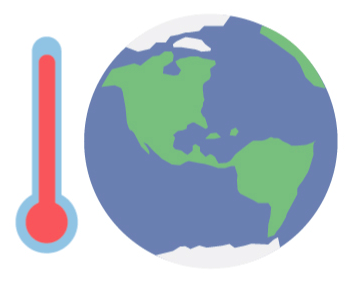
\includegraphics[width=3.2cm]{"Images_intro/earth.png"}};}
    
    \onslide<2-8>{\draw[line width=6pt,purple,-{Triangle[width=1.8*6pt,length=0.8*6pt,purple]}](ff) to [out=135,in=300] (pmm);}
    \onslide<2-8>{\draw[line width=6pt,purple,-{Triangle[width=1.8*6pt,length=0.8*6pt,purple]}](ff) to [out=45,in=225] (oo);}
    \onslide<3-8>{\draw[line width=6pt,purple,-{Triangle[width=1.8*6pt,length=0.8*6pt,purple]}](ff) to [out=280,in=200] (ghg);}
    \onslide<4-8>{\draw[line width=6pt,purple,-{Triangle[width=1.8*6pt,length=0.8*6pt,purple]}](ghg) to [out=15,in=260] (earth);}
    
    % decrease arrow
    \onslide<5-8>{\draw[line width=6pt,green,-{Triangle[width=1.8*6pt,length=0.8*6pt,green]}](9.15,0) to (9.15,-2);}
    \onslide<6-8>{\draw[line width=6pt,green,-{Triangle[width=1.8*6pt,length=0.8*6pt,green]}](6.5,-3) to (6.5,-5);}
    \onslide<7-8>{\draw[line width=6pt,green,-{Triangle[width=1.8*6pt,length=0.8*6pt,green]}](2.45,-1) to (2.45,-3);}
    \onslide<8-8>{\draw[line width=6pt,green,-{Triangle[width=1.8*6pt,length=0.8*6pt,green]}](1,1.5) to (1,0.5);}
    \onslide<8-8>{\draw[line width=6pt,green,-{Triangle[width=1.8*6pt,length=0.8*6pt,green]}](6,1.5) to (6,0.5);}
\end{tikzpicture}
\end{frame}

\begin{frame}
\frametitle{\pmm\ map}
\centering
\href{https://www.iqair.com/earth}{\textcolor{blue}{\pmm\ map}}
\href{https://www.iqair.com/earth}{(\textcolor{blue}{https://www.iqair.com/earth})}
\end{frame}

\begin{frame}
\frametitle{Health impact of \pmm}
\begin{figure}
    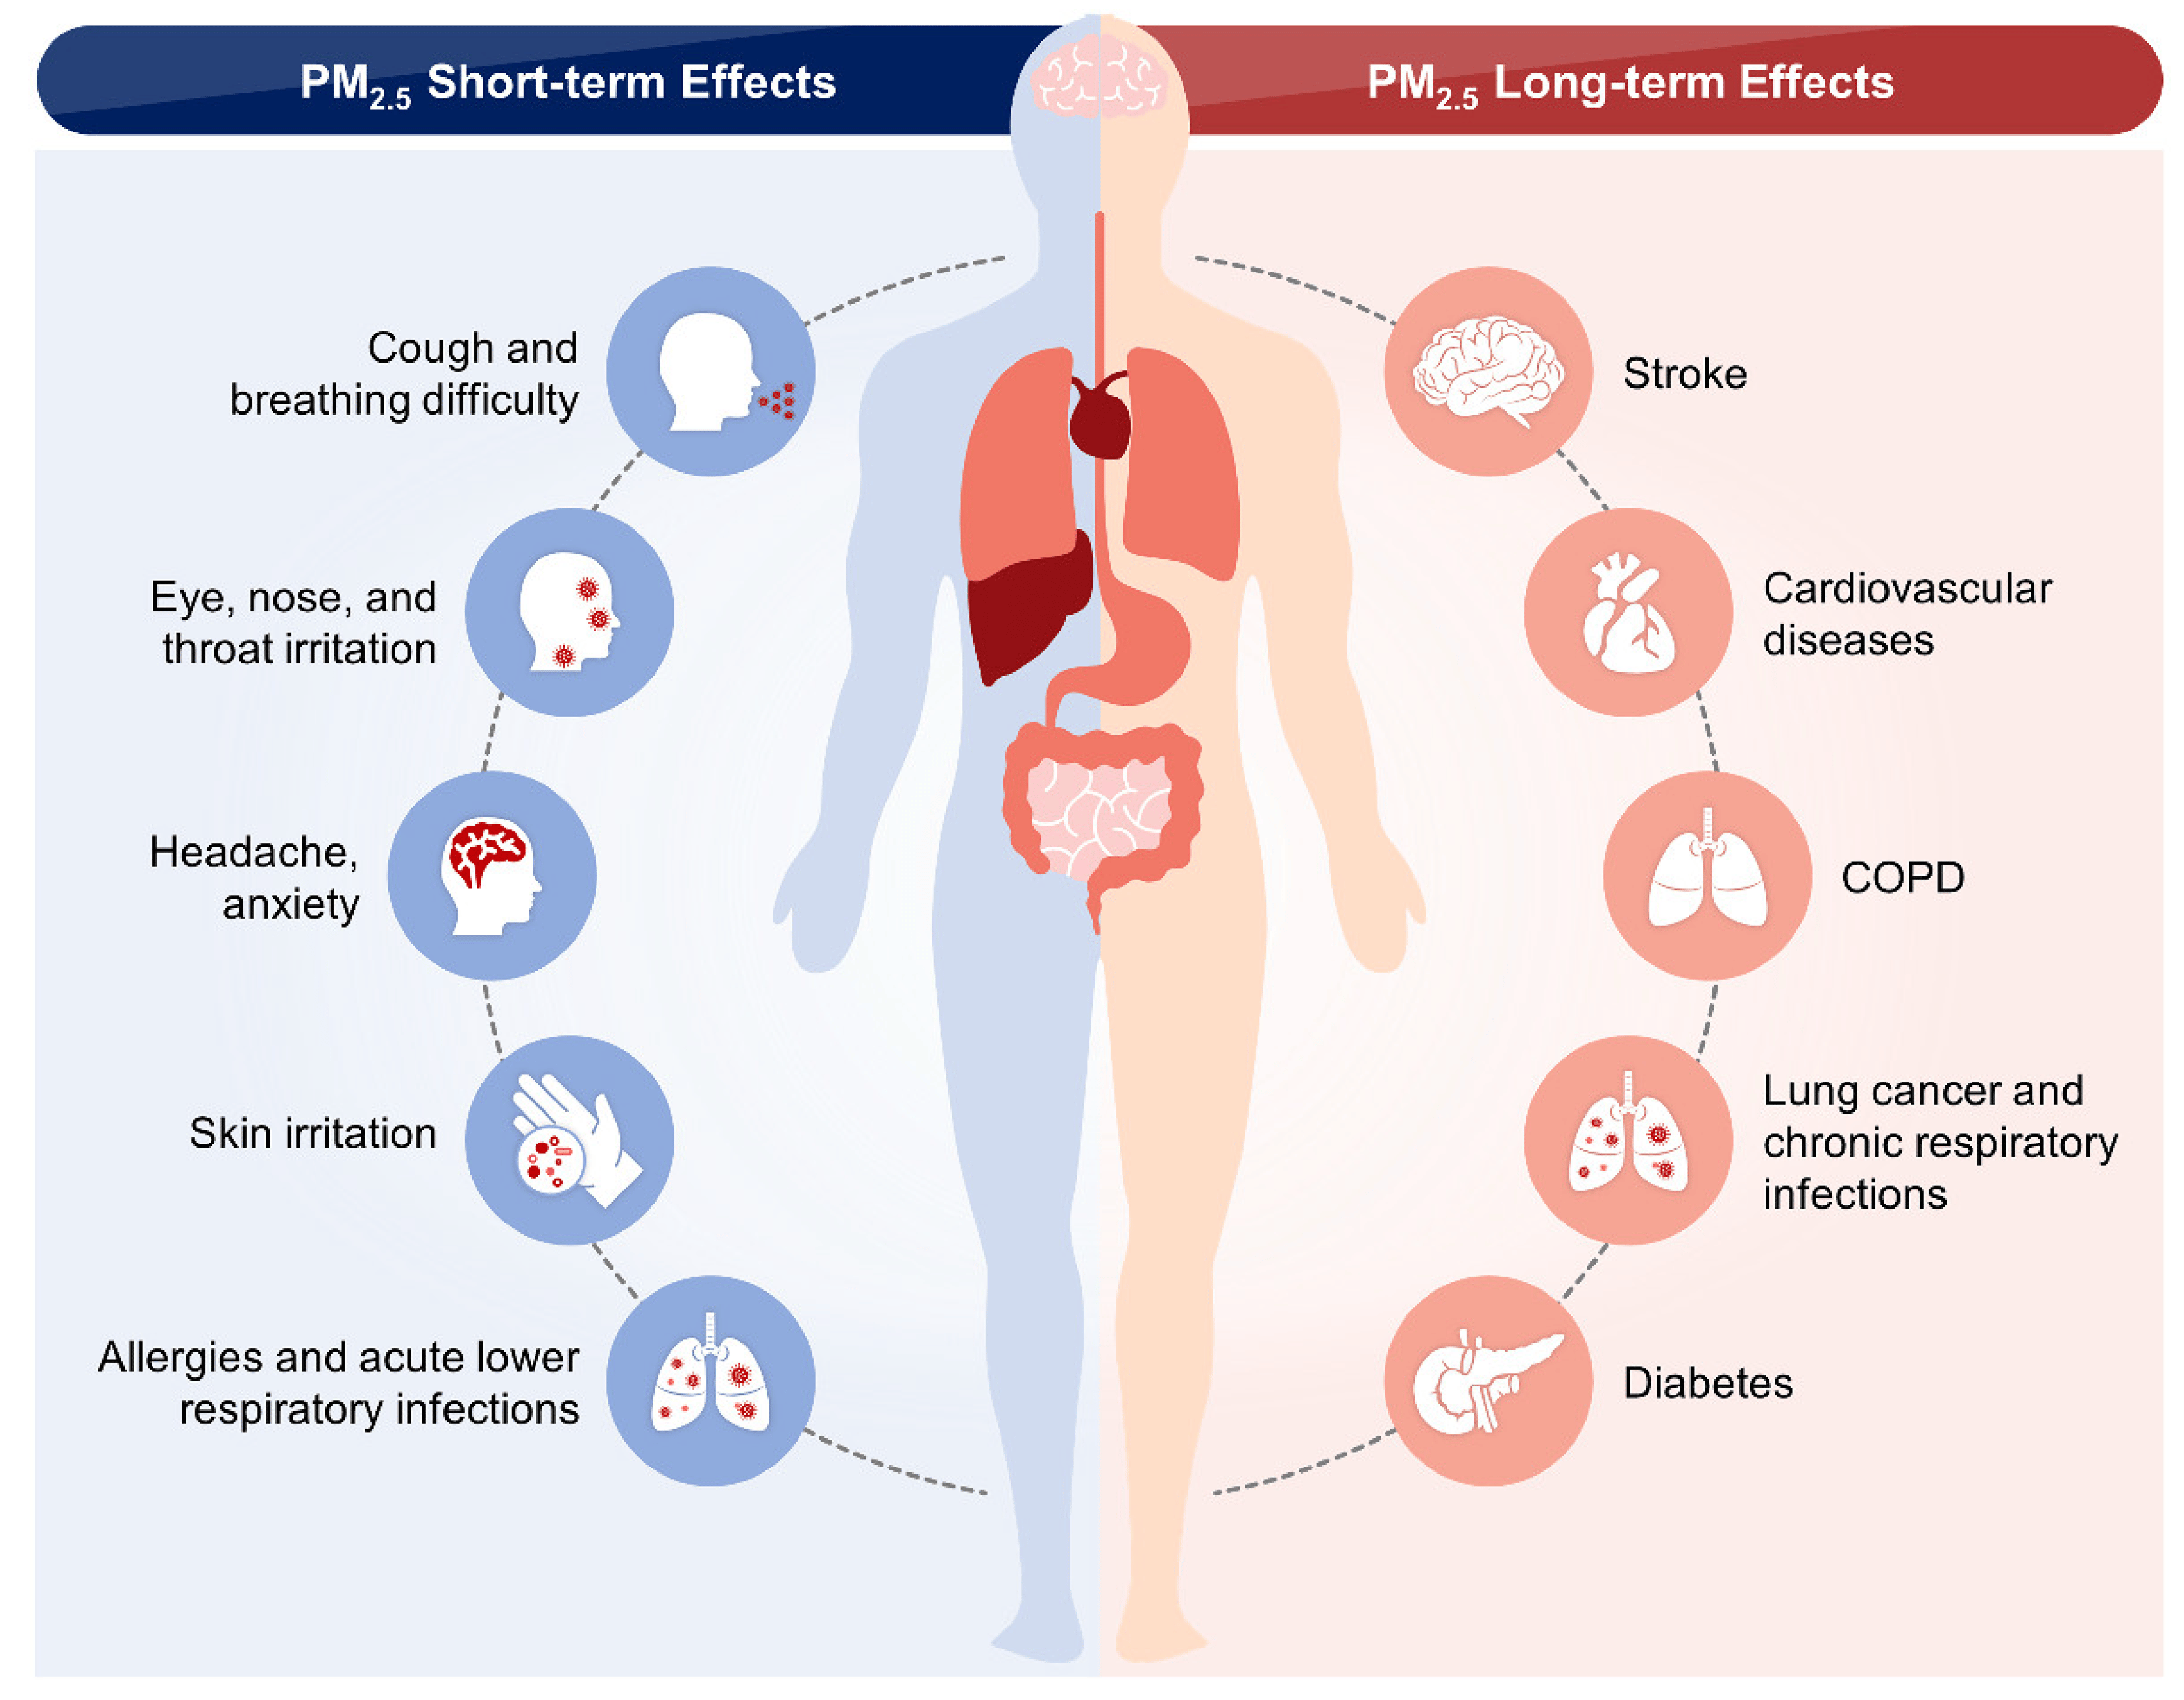
\includegraphics[width = 0.8\linewidth]{Images_intro/pm_impacts.png}
\end{figure}
\vfill \hfill \tiny{\cite{basith_impact_2022}}
\end{frame}

\begin{frame}
\frametitle{Health impacts of \pmm\ \& \oo}
\centering
\href{https://vizhub.healthdata.org/gbd-compare/}{\textcolor{blue}{IHME database}}
\href{https://vizhub.healthdata.org/gbd-compare/}{(\textcolor{blue}{\texttt{https://vizhub.healthdata.org/gbd-compare/}})}
\end{frame}


\begin{frame}
\frametitle{Air pollution health and economic implications}
\begin{itemize}
    \setlength\itemsep{0.3cm}
    \item Premature deaths
    \item Years of Life Lost (YLLs)
    \item Disability Adjusted Life Years (DALYs)
    \item ...
\end{itemize}
\vspace{0.35cm}
\begin{center}
\pause\text{\Large$ \Downarrow $}
\end{center}
\vspace{0.35cm}
\begin{itemize}
    \setlength\itemsep{0.3cm}
    \item Economy growth
    \item Human Capital Lost (HCL)
    \item Value of Statistical Life (VSL)
    \item ...
\end{itemize}
\end{frame}

